The discrete twinning model incorporates a spatially resolved representation of twinning events, aligning with experimental observations. Unlike volume fraction-based approaches where material points can simultaneously exhibit both twinned and untwinned states, the discrete model restricts each point to either the twinned or untwinned (parent) state similar to an order parameter in phase field modelling.

This discrete twinning model can couple with existing crystal plasticity formulations in the multiphysics DAMASK simulation package \cite{ROTERS2019420}. While the crystal plasticity component handles deformation from dislocation slip, the discrete twinning portion specifically captures the mechanical twinning contribution. By segregating the slip and twinning behaviours, the model provides more physical fidelity and flexibility compared to conventional phenomenological implementations. Overall, the discrete twinning approach enables targeted insights into the distinct twinning phenomenology while seamlessly integrating with DAMASK's extensive crystal plasticity multi-physics modelling capabilities.

\section{Assumptions made in the discrete twinning model.}

\begin{itemize}
\item Grain boundaries are assumed to be the location of nucleation events.
\item We consider all the discretized material points (FFT voxel or FEM element) which are neighbouring to twinned elements for growth of the twin.
\item All the discretized material points which are considered for nucleation or growth are assigned a random number. The random number assigned is uniformly distributed between 0 and 1.
\item Since twinning frequency and variant selection frequency are strongly correlated with Schmid factor, we consider volume fraction which is derived using Schmid factor as the criteria for declaring the discretized material point as discretely twinned. 
\item The twin events are considered as instantaneous and the discretized material point is flipped at the same time step.


\end{itemize}

\section{Incorporating the stochastic nature of the deformation twins.}

As we have seen in the literature review section \ref{Stochastic_nature}, deformation twinning is inherently stochastic process, and to model this we use random sampling technique inspired by the Monte Carlo Method.

\subsection{The Monte Carlo method}

Monte Carlo methods are widely used computational techniques that estimate solutions to problems that are challenging or impractical to solve using deterministic methods. They achieve this by employing repeated random sampling, drawing randomly generated numbers as inputs to simulate a wide range of potential outcomes.

In Monte Carlo methods, randomness is used to provide estimates of deterministic quantities. A simple application of this numerical technique is the estimation of the area between two curves.

Consider the following two curves: \\
Curve 1: $y = 2x$ \\
Curve 2: $y = x^2$

To estimate the area between these two curves using the Monte Carlo method, we first define the limits of the region (the bounding rectangle) that encloses the area of interest. In this case, the limits are set to $x_{min} = 0,\ x_{max} = 2,\ y_{min} = min(func1(x_{min}),\ func2(x_{min})),$ and $y_{max} = max(func1(x_{max}),\ func2(x_{max}))$.

The Monte Carlo simulation is performed by generating a large number of random points within the bounding rectangle domain. For each random point, we check if it falls within the area between the two curves by evaluating the conditions: $ y_{min} \leq y \leq max(func1(x),\ func2(x)) $ and $ min(func1(x),\ func2(x)) \leq y $.

\begin{figure}[H]
  \centering
  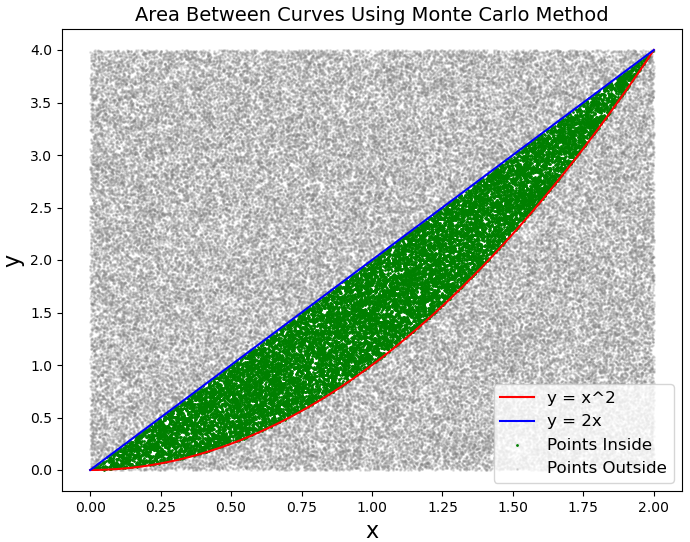
\includegraphics[width=0.6\textwidth]{images/monte_carlo_area.png}
  \caption{Simple application of monte carlo method}
  \label{Monte_carlo_app}
\end{figure}


The ratio of points inside the area to the total number of points, multiplied by the area of the bounding rectangle, gives an estimate of the area between the curves.
\[
\textbf{Area\ between\ the\ curves} = \frac{Points\ inside\ the\ area}{Total\ number\ of\ points} * {Area\ of\ the\ bounding\ rectangle}
\]
The accuracy of the estimated area depends on the number of random points generated. Increasing the number of points will generally lead to a more accurate estimate, but it will also increase the computation time.

\subsection{Random sampling technique applied in the discrete twin model.}
The twinning is inherently stochastic in nature; we introduce stochasticity to our model using a random sampling method (similar to Monte Carlo method) to determine if a particular material point is activated for twin nucleation or growth. At each time step all the material points in the parent crystal are assigned a random number between 0 and 1. For each material point where the random number is compared using a predefined criteria. Based on the outcome of this, the material point is given a discrete state of twinning: either twinned or not twinned. The criteria we use is the local stress-driven evolution of the twin volume fraction for a specific twin system, obtained per the equation from Kalidindi's model \cite{KALIDINDI1998267}:

\[
\dot{f}_\text{twin}^\beta = 
\begin{cases}
\dot{\gamma}_0 \left(\lvert \tau^\beta \rvert/\tau^{\beta}_c\right)^n/\gamma^c_\text{twin} & \text{if } \tau^\beta > 0 \\\\
0 & \text{if } \tau^\beta \leq 0
\end{cases}
\]

where $\tau^{\beta}$ , $\tau_c^{\beta}$ , $\gamma_{twin}^c$ represent stress driving force, critical resolved shear stress (CRSS) for twinning and characteristic shear due to mechanical twinning.

If the sampling outcome is “failure," no changes occur and sampling continues. If the outcome is “success," the material point state flips immediately to the twinned state, the consequences of which are discussed in section .

\subsection{Sampling parameters.}
\subsubsection{Frequency of sampling.}

 \begin{figure}[H]
    \centering
    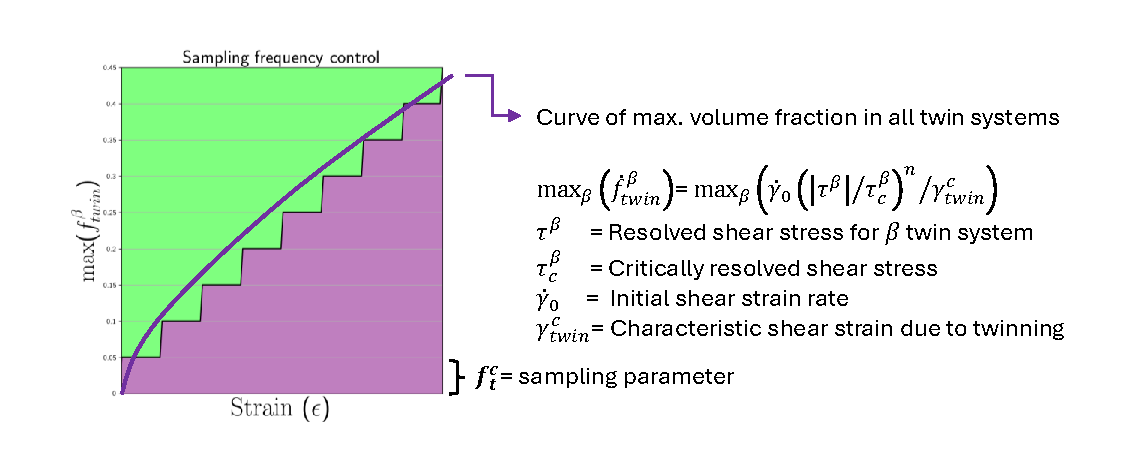
\includegraphics[width=\textwidth]{images/Sampling_parameter.pdf}
    \caption{Scheme to control sampling frequency.}
    \label{Sampling_frequency}
\end{figure}

 If a voxel is sampled more times it has more chances of getting twinned. In other words, Frequency of sampling of the voxel determines probability of twinning. In the discrete twin model, if a voxel is sampled once, we make it harder for it to sample it again by increasing a parameter. This follows the evolution of the maximum volume fraction of all the twin systems. The schematic representation of this is given in figure \ref{Sampling_frequency}.
 
\subsubsection{Distribution of random number.}
 The distribution or range of the random number can be regulated relative to the volume fraction to control the onset of sampling. For instance, if the range of random numbers is restricted between 0.4 and 1, then sampling will only commence after the volume fraction reaches 0.4 for the voxel. This is analogous to expanding or contracting the domain over which random sampling occurs. It resembles adjusting the size of the bullseye in a dart game.

\subsection{Separate treatment of nucleation and growth of twins.}

\begin{wrapfigure}{rH}{0.45\textwidth}
    \centering 
    \resizebox{0.4\textwidth}{!}{
    \includesvg[width=0.4\textwidth]{images/Twin_events_schematic.svg}}
    \caption{Twinning events schematic.}
    \caption*{\ \ First a grain boundary element is twinned and neighbouring elements are selected for growth. For thickening of twin, subsequent neighbours are selected.}
    \label{fig:Twinning_events}
\end{wrapfigure}

We treat nucleation and growth events separately.

The nucleation events are assumed to happen at grain boundaries following the work of Beyerlein(2010) \cite{beyerlein2010probabilistic}. Nucleation occurs independently at grain boundaries, with volume fraction driven by local stress as the sole criteria for event initiation.

The growth events which includes propagation and band thickening is done by method similar to Cheng(2017) \cite{CHENG2017512}, where neighbouring elements are identified and the maximum volume fraction of all twin systems is compared with the random number assigned for that voxel. Growth only proceeds if at least one neighboring point is already twinned, making neighbor state (twinned or untwinned) which is decided by random sampling parameters.

\subsubsection{Selection of Neighbouring Voxels/Elements.}
We select neighbouring voxels using a ``do" loop which loops from ONE to total number of neighbours. In a structured hexahedral grid, the number of neighbours adjacent to 6 faces of element are 6, the loop runs from 1 to 6. ``IPneighborhood" function provided in the DAMASK is used to identify all the neighbouring elements and element number is assigned to a local variable. This element number is then used to obtain information about the voxel like highest twin volume fraction and respective variant.

\subsection{Defining a ``success" event}
\label{consequence_of_success}
If a voxel passes all the criteria, it is consider ``twinned" we update a logical flag ``twinJump" as .true. We also update the variable $\Delta F_p$ with the correspondence matrix of the respective twin system. The entire process is given in the flow chart below along with the source code.

\begin{figure}[H]
    \centering
    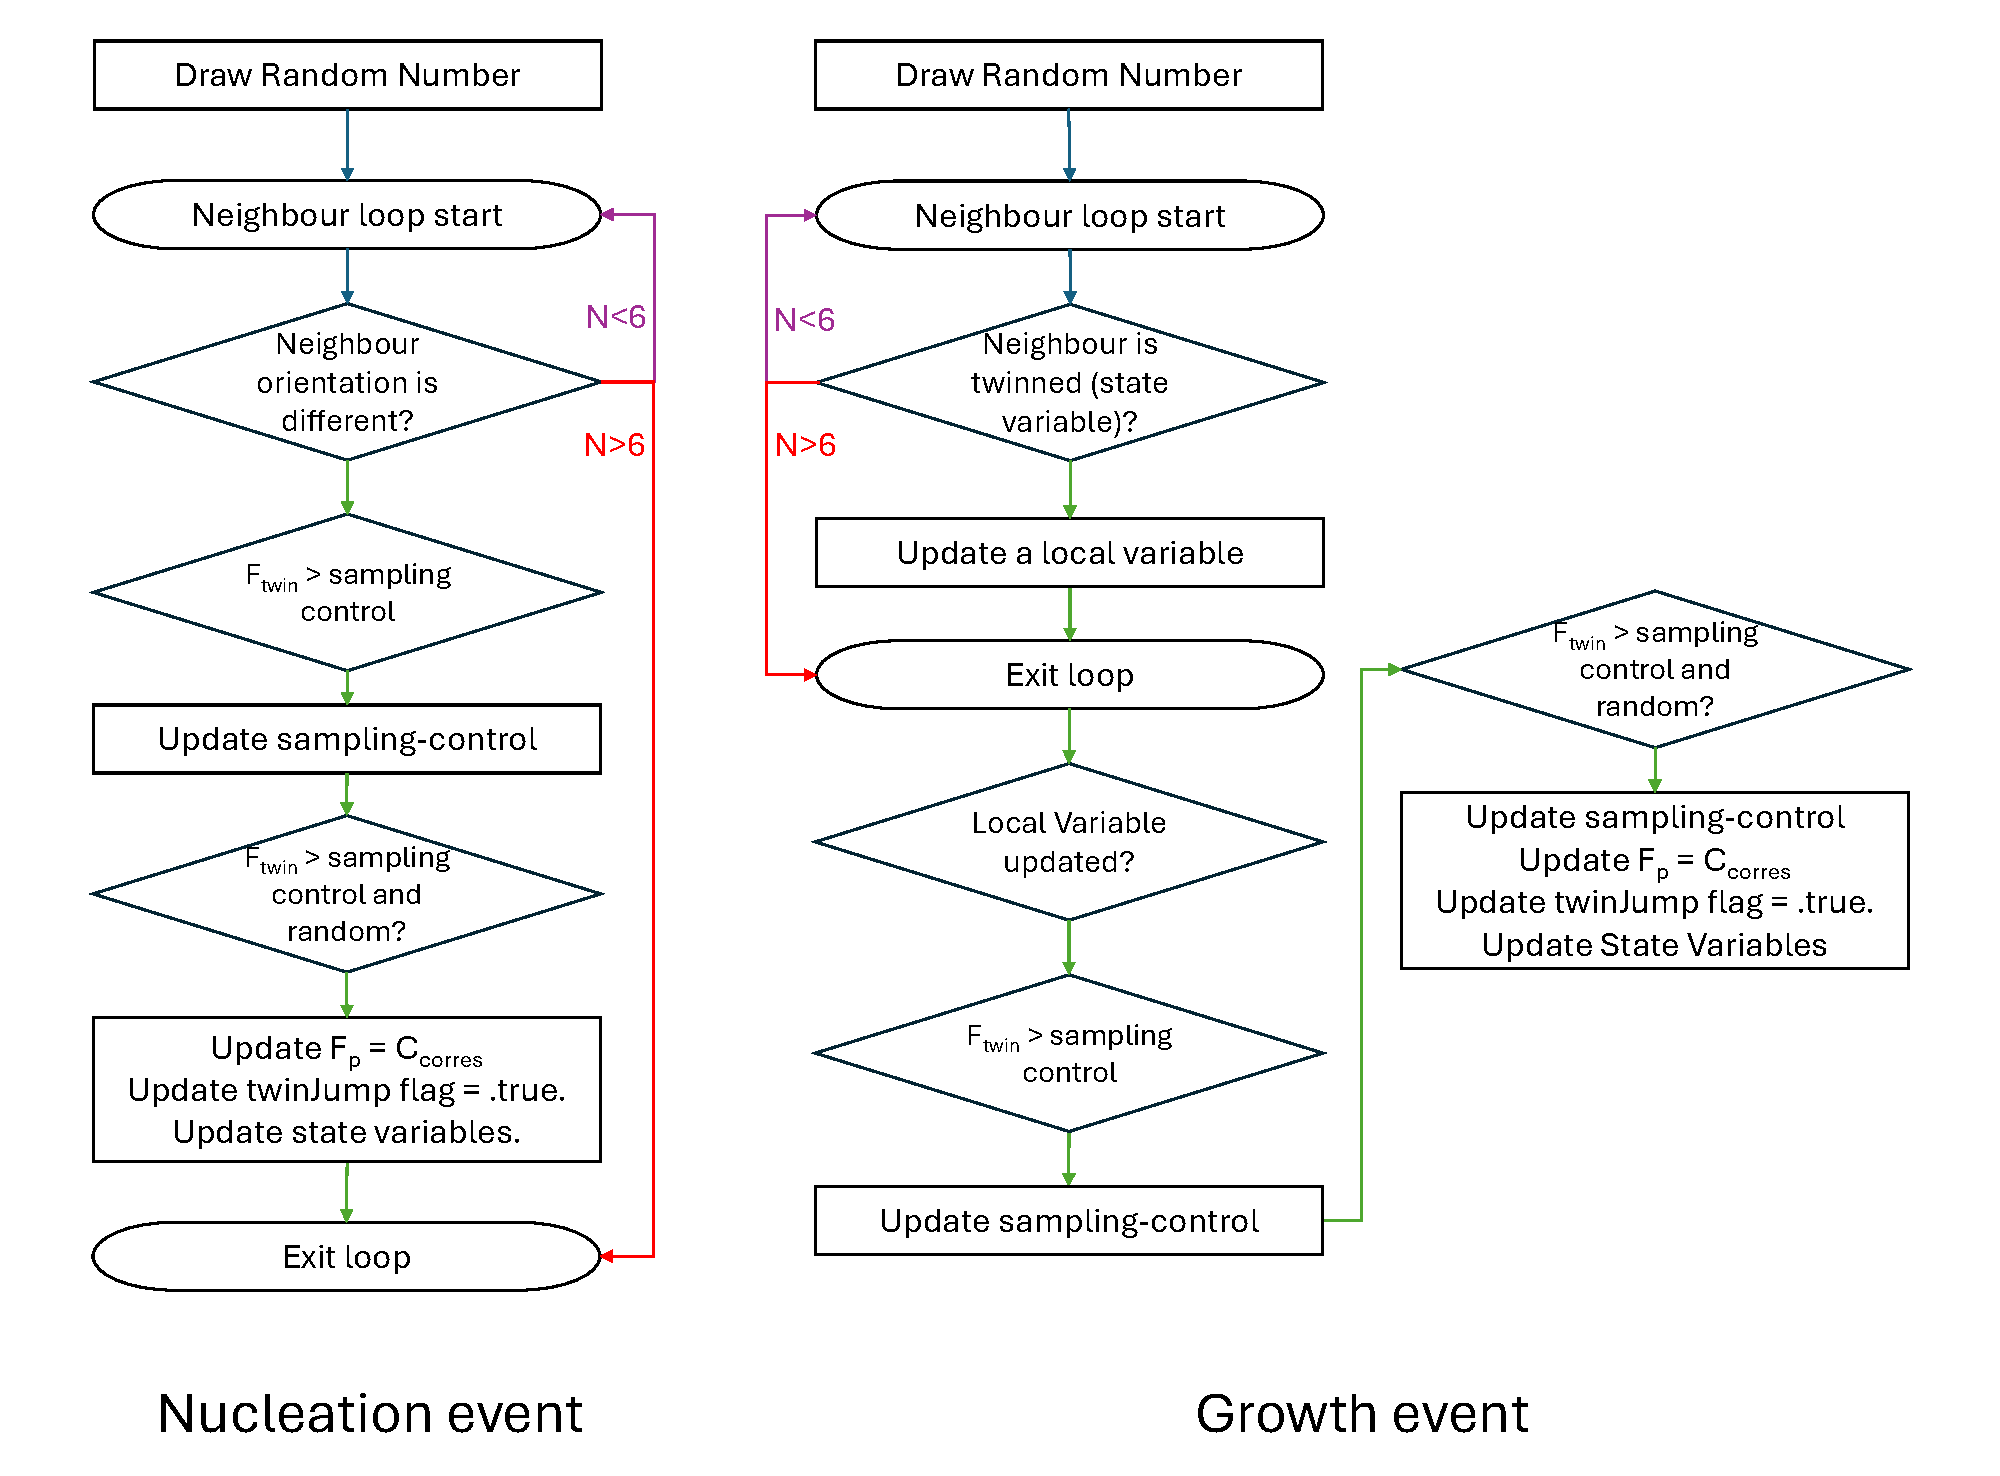
\includegraphics[width=\textwidth]{images/Flow_chart_twin_events.pdf}
    \caption{Initiation of twinning events at a material point.}
    \label{Flow_chart_twin_events}
\end{figure}


\begin{minted}[fontsize=\scriptsize, frame=single]{fortran}
!--------------------------------------------------------------------------------------------
!> @brief calculates instantaneous incremental change of kinematics and associated jump state
!> Satya, Achal
!--------------------------------------------------------------------------------------------
module subroutine plastic_kinematic_deltaFp(ph,en,twinJump,deltaFp)

integer,                     intent(in)  :: &
  ph, &
  en
logical,                     intent(out) :: &
  twinJump
real(pREAL), dimension(3,3), intent(out) :: &
  deltaFp  
integer :: &
  n, &                                               ! neighbor index
  neighbor_e, &                                      ! element index of my neighbor
  neighbor_ip, &                                     ! integration point index of my neighbor
  neighbor_en, &
  neighbor_ph
real(pREAL) :: &
  random, random_g, &
  nRealNeighbors
integer :: &
  twin_var, var_growth
real(pREAL), dimension(param(ph)%sum_N_tw)  :: &
  fdot_twin
real(pREAL), dimension(param(ph)%sum_N_tw)  :: &
  tau_tw
integer :: i

twinJump = .false.
deltaFp = math_I3
  
associate(prm => param(ph), stt => state(ph), dlt => deltastate(ph))
  twin_var = maxloc(stt%f_twin(:,en),dim=1)

  Discrete_twin: if ( prm%discrete_twin ) then
  Frozen: if(stt%frozen(en)<1.0_pREAL) then
    
  call random_number(random)
  call random_number(random_g)
    
  do n = 1, ncellneighbors
    neighbor_e = geom(ph)%IPneighborhood(1,n,en)                   !< Identify neighbor
    !< Identify grain boundary elements
    if (any(dNeq(phase_O_0(ph)%data(en)%asQuaternion(),&
        phase_O_0(ph)%data(neighbor_e)%asQuaternion()))) then       
      Ability_Nucleation: if(stt%f_twin(twin_var,en)> &
                            (stt%fmc_twin(twin_var,en)+ &
                            prm%checkstep(twin_var))) then          !< Frequency control
        stt%fmc_twin(twin_var,en) = stt%fmc_twin(twin_var,en) &
                                  +prm%checkstep(twin_var)
        Success_Nucleation: if (random <= stt%f_twin(twin_var,en)) then          
          twinJump = .true.
          deltaFp  = prm%CorrespondenceMatrix(:,:,twin_var)
          exit
        endif Success_Nucleation
      endif Ability_Nucleation
    endif
  end do

  NeighborLoop: do n = 1, ncellneighbors
    neighbor_e = geom(ph)%IPneighborhood(1,n,en)
    if(stt%variant_twin(neighbor_e)>0) then                    !< Check if neighbor is twinned
      var_growth = stt%variant_twin(neighbor_e)
      exit NeighborLoop
    endif
  enddo NeighborLoop

  Growth_Criteria: if(var_growth>0.0_pReal) then                     !< If neighbor twinned,
    Ability_Growth: if(stt%f_twin(twin_var,en) &
                       >(stt%fmc_twin(twin_var,en) &
                          +prm%checkstep(twin_var))) then            !< Frequency control
      stt%fmc_twin(twin_var,en) = stt%fmc_twin(twin_var,en) &
                                  +prm%checkstep(twin_var)
      Success_Growth: if (0.3_pREAL+random_g*0.7_pREAL 
                           <= stt%f_twin(twin_var,en)) then          !< Random sampling
        twinJump = .true.                                            !< Output flag
        deltaFp  = prm%CorrespondenceMatrix(:,:,twin_var)            !< Correspondence Matrix
      endif Success_Growth
    endif Ability_Growth
  endif Growth_Criteria
  
  endif Frozen
  end if Discrete_twin
end associate
  
end subroutine plastic_kinematic_deltaFp
\end{minted}


\section{Handling of twinning and slip in the kinematics.}

\subsection{Consequences of a “Success” event in Sampling Outcome:}
The impacts of Monte-Carlo “success” are equivalent for nucleation and growth, triggering a flip from the parent to the twinned state. This transformation follows the correspondence matrix formulation discussed earlier. The matrix combines the twinning shear (S) and lattice rotation (U) of mechanical twinning.

\subsection{The Twinning Jump.}
The primary consequence of a parent-to-twin flip is a sudden jump in the plastic deformation gradient Fp, arising from twinning-induced rotation and shear. This contrasts the typical gradual Fp rate evolution from crystal plasticity dislocation slip, as shown in Figure \ref{fig: Kinematic_jump}.
\begin{figure}[H]
    \centering
    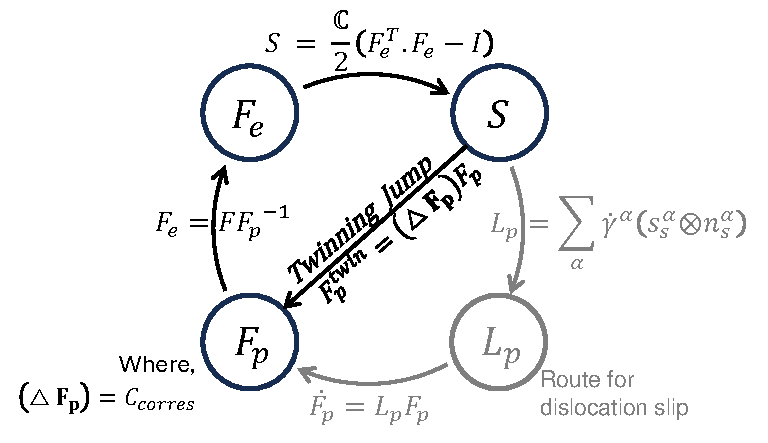
\includegraphics[width=0.7\textwidth]{images/Kinematic_Jump.pdf}
    \caption{Twinning kinematic framework.}
    \label{fig: Kinematic_jump}
\end{figure}
\subsubsection{The ``delta state".}
It is necessary to express the change in the state in terms of an instantaneous jump rather as rate of change. Here we device a rate independent constitutive description.
We treat deformation twinning as a instantaneous jump and in the DAMASK the variables related to deformation twinning are undated in the ``delta state".

We use 4 delta state variables which defines the micro structure parameters.
\begin{enumerate}
    \item f\_twin : Variable used for the random sampling criteria.
    \item fmc\_twin : Variable used for the sampling frequency control.
    \item frozen or f\_binary \\ Discrete quantity which assumes either +1 or -1. It is also used to freeze the voxel so that it is not available for deformation by slip or twinning.
    \item variant\_twin : Used to store the variant of the twin.
\end{enumerate}

\begin{minted}[fontsize=\scriptsize, frame=single]{fortran}
!-------------------------------------------------------------------
!> @brief calculates (instantaneous) incremental change of 
!> microstructure
!> Satya, Achal
!-------------------------------------------------------------------
module subroutine plastic_phenopowerlaw_deltaState(ph,en)
  implicit none
  integer, intent(in)::&
    ph, &
    en
  logical :: &
    twinJump
  integer :: &
    twin_var
  real(pREAL), dimension(3,3) :: &
    deltaFp
    
  associate(prm => param(ph), stt => state(ph), dlt => deltastate(ph))
    twin_var = maxloc(stt%f_twin(:,en),dim=1)
    call plastic_kinematic_deltaFp(ph,en,twinJump,deltaFp)
      if(twinJump) then
        dlt%f_twin(:,en)     = 0.0_pReal - stt%f_twin(:,en)
        dlt%fmc_twin(:,en)   = 0.0_pReal - stt%fmc_twin(:,en)
        dlt%frozen(en)       = 1.0_pReal - stt%frozen(en)
        dlt%variant_twin(en) = twin_var 
      else
        dlt%f_twin(:,en)     = 0.0_pReal
        dlt%fmc_twin(:,en)   = 0.0_pReal
        dlt%frozen(en)       = 0.0_pReal
        dlt%variant_twin(en) = 0.0_pREAL
      endif
  end associate
  
  end subroutine plastic_phenopowerlaw_deltaState
\end{minted}

The delta state variables which sits at the end of the global container will update the state variable at the given time step explicitly.

\subsection{Correspondence matrix.}
\begin{wrapfigure}{rH}{0.35\textwidth}
    \centering 
    \resizebox{0.35\textwidth}{!}{
    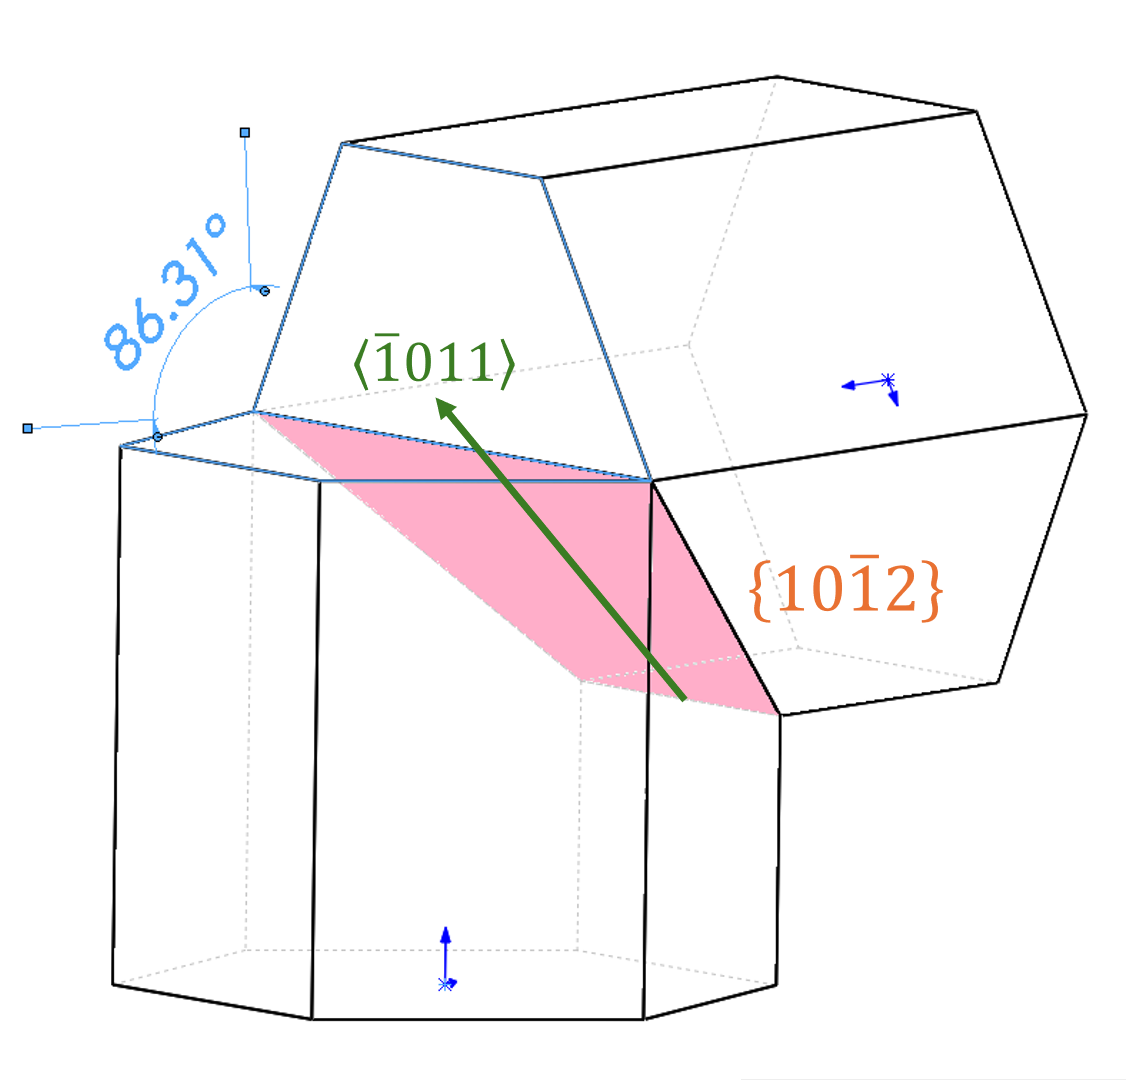
\includegraphics[width=0.5\textwidth]{images/Extension_twin_crystallography.png}}
    \caption{Extension twin crystallography replicated using 3D CAD model in \textbf{SolidWorks}.}
    \label{Extension twin crystallography}
\end{wrapfigure}

When twinning occurs, the parent crystal is sheared and reoriented. The misorientation in two lattices is the unique for a particular twinning mode. For example, $(\bar{1}012)[10\bar{1}1]$ twinning mode in Mg with c/a ratio 1.624 can be recognized by the unique misorientation of 86.31 degrees angle between c-axis in the parent and twin.

This is shown in the figure \ref{Extension twin crystallography} where we take 2 hexagonal lattices with c/a ratio of 1.624 in a CAD software like \textbf{Solidworks}. We then cut it in $(\bar{1}012)$ plane and assemble the lattices in $[10\bar{1}1]$ direction and measure the angle between the corresponding faces of parent and twin. The measured angle gives the unique misorientation angle which is 86.31 degrees.

This crystallographic transformation is mathematically described by the correspondence matrix given by Niewczas \cite{Niewczas121}. Correspondence matrix gives equation for transformation of vector or a plane in parent lattice to twinned lattice. Correspondence matrix provides essential means to predict the physical transformation of crystallographic directions and planes resulting from twinning. Appendix \ref{Appendix:Correspondence_matrix} has more details about the correspondence matrix approach.

\subsection{Incorporating Large deformation caused by Twinning.}

\begin{figure}[H]
    \centering
    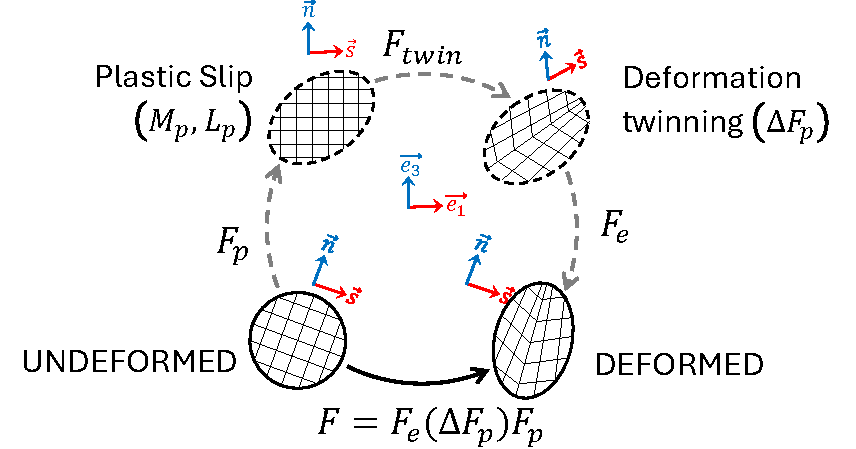
\includegraphics[width=0.55\textwidth]{images/Delta_twin_as_Intermediate_configuration.pdf}
    \caption{Delta State of Twinning as intermediate configuration.}
    \caption*{\ \ Taking ${F_p}_{(t=0)} = O_0$ so that lattice coordinates $\hat{n}$,$\hat{s}$ coincide with lab coordinate system $\overrightarrow{e_3}$,$\overrightarrow{e_1}$ }
    \label{fig:DeltaStateIntermediateConfig}
\end{figure}

In the single constituent kinematics, clear distinction is made between different deformation modes: Elastic deformation and Plastic Deformation and within the plastic deformation modes: Slip and Twinning. Twinning which causes sudden change in the shear and it reorients the lattice. Hence, is not evaluated along with the slip but it is pre-multiplied to the plastic deformation gradient. The above figure \ref{fig:DeltaStateIntermediateConfig} shows how both the shear and reorientation are introduced in the lattice.

\begin{figure}[H]
    \centering
    \fbox{\resizebox{0.6\textwidth}{!}{
    \begin{circuitikz}
\tikzstyle{every node}=[font=\LARGE]
\draw  (22.5,30.5) rectangle (30,21.75);
\draw [short] (23.75,30.5) -- (23.75,21.75);
\draw [short] (25,30.5) -- (25,21.75);
\draw [short] (26.25,30.5) -- (26.25,21.75);
\draw [short] (27.5,30.5) -- (27.5,21.75);
\draw [short] (28.75,30.5) -- (28.75,21.75);
\draw [short] (22.5,29.25) -- (30,29.25);
\draw [short] (22.5,28) -- (30,28);
\draw [short] (22.5,26.75) -- (30,26.75);
\draw [short] (22.5,25.5) -- (30,25.5);
\draw [short] (22.5,24.25) -- (30,24.25);
\draw [short] (22.5,23) -- (30,23);

% Sheared config

\draw [short] (21.25,8) -- (22.5,16.75);
\draw [short] (21.25,8) -- (28.75,8);
\draw [short] (28.75,8) -- (30,16.75);
\draw [short] (22.5,16.75) -- (30,16.75);

\draw [short] (22.33,15.5) -- (29.83,15.5);
\draw [short] (22.15,14.25) -- (29.65,14.25);
\draw [short] (21.97,13) -- (29.47,13);
\draw [short] (21.79,11.75) -- (29.29,11.75);
\draw [short] (21.61,10.5) -- (29.11,10.5);
\draw [short] (21.43,9.25) -- (28.93,9.25);

\draw [short] (22.5,16.75) -- (22.5,8);
\draw [short] (23.75,16.75) -- (23.75,8);
\draw [short] (25,16.75) -- (25,8);
\draw [short] (26.25,16.75) -- (26.25,8);
\draw [short] (27.5,16.75) -- (27.5,8);
\draw [short] (28.75,16.75) -- (28.75,8);

%Twinned config

\draw [short] (40,16.75) -- (47.5,16.75);
\draw [short] (36.25,8) -- (43.75,8);
\draw [short] (39.4,15.5) -- (46.9,15.5);
\draw [short] (38.75,14.25) -- (46.25,14.25); 
\draw [short] (36.9,9.25) -- (44.4,9.25);
\draw [short] (37.5,10.5) -- (45,10.5);

\draw [short] (46.25,16.75) -- (46.25,14.25);
\draw [short] (45,16.75) -- (45,14.25);
\draw [short] (43.75,16.75) -- (43.75,14.25);
\draw [short] (42.5,16.75) -- (42.5,14.25);
\draw [short] (41.25,16.75) -- (41.25,14.25);
\draw [short] (40,16.75) -- (40,14.25);
%\draw [short] (38.75,16.75) -- (38.75,14.25);
\draw [short] (43.75,10.5) -- (43.75,8);
\draw [short] (42.5,10.5) -- (42.5,8);
\draw [short] (41.25,10.5) -- (41.25,8);
\draw [short] (40,10.5) -- (40,8);
\draw [short] (38.75,10.5) -- (38.75,8);
\draw [short] (37.5,10.5) -- (37.5,8);
%\draw [short] (36.25,10.5) -- (36.25,8);


\draw [short] (43.75,10.5) -- (45,14.25);
\draw [short] (42.5,10.5) -- (43.75,14.25);
\draw [short] (41.25,10.5) -- (42.5,14.25);
\draw [short] (40,10.5) -- (41.25,14.25);
\draw [short] (38.75,10.5) -- (40,14.25);
\draw [short] (37.5,10.5) -- (38.75,14.25); % left edge y = 3 x - 102
%\draw [short] (36.25,10.5) -- (37.5,14.25);
\draw [short] (45,10.5) -- (46.25,14.25); % right edge y = 3 x - 124.5

\draw [short] (38.625,13.875) -- (45.375,11.625); %x = 45.375 and y = 11.625, x = 38.625 and y = 13.875
\draw [short] (41.25,14.25) -- (45.75,12.75); % x = 45.75 and y = 12.75
\draw [short] (45,14.25) -- (46.125,13.875); % x = 46.125 and y = 13.875
\draw [short] (38.25,12.75) -- (45,10.5); % x = 38.25 and y = 12.75
\draw [short] (37.875,11.625) -- (41.25,10.5); %x = 37.875 and y = 11.625

\draw [short] (43.75,8) -- (45,10.5);
\draw [short] (46.25,14.25) -- (47.5,16.75);
\draw [short] (36.25,8) -- (37.5,10.5);
\draw [short] (38.75,14.25) -- (40,16.75);


%Final config

\draw [short] (38.022,28.218) -- (39.000,30.500); % left vertical
\draw [short] (36.708,21.985) -- (45.458,23.208); % bottom horizontal
\draw [short] (39.000,30.500) -- (47.750,31.750);  % top
\draw [short] (46.772,29.468) -- (47.750,31.750); % right
\draw [short] (45.947,24.350) -- (37.191,23.099); % 
\draw [short] (46.437,25.491) -- (37.687,24.241); % bottom 2
\draw [short] (38.511,29.359) -- (47.261,30.609); % 
\draw [short] (38.022,28.218) -- (46.772,29.468); %top 2

\draw [short] (37.687,24.241) -- (36.708,21.985);%
\draw [short] (39.145,24.449) -- (38.167,22.167);% bott
\draw [short] (40.603,24.658) -- (39.625,22.375);%
\draw [short] (42.062,24.866) -- (41.083,22.583); % 
\draw [short] (43.520,25.074) -- (42.542,22.792); % 
\draw [short] (44.978,25.283) -- (44.0,23);
\draw [short] (46.437,25.491) -- (45.458,23.208);

\draw [short] (39.480,28.426) -- (40.458,30.708);
\draw [short] (40.939,28.634) -- (41.917,30.917);
\draw [short] (42.397,28.843) -- (43.375,31.125); % tops
\draw [short] (43.855,29.051) -- (44.833,31.333);
\draw [short] (45.313,29.259) -- (46.292,31.542);

\draw [short] (37.687,24.241) -- (38.022,28.218); %Twin
\draw [short] (39.145,24.449) -- (39.480,28.426); %2
\draw [short] (40.603,24.658) -- (40.939,28.634); %3
\draw [short] (42.062,24.866) -- (42.397,28.843);
\draw [short] (43.520,25.074) -- (43.855,29.051);
\draw [short] (44.978,25.283) -- (45.313,29.259);
\draw [short] (46.437,25.491) -- (46.772,29.468);

\draw [short] (45.313,29.259) -- (46.687,28.466);
\draw [short] (43.855,29.051) -- (46.604,27.474);
\draw [short] (42.397,28.843) -- (46.520,26.483);
\draw [short] (40.939,28.634) -- (46.437,25.491);
\draw [short] (39.480,28.426) -- (44.978,25.283);
\draw [short] (38.022,28.218) -- (43.520,25.074);
\draw [short] (37.939,27.226) -- (42.062,24.866);
\draw [short] (37.855,26.235) -- (40.603,24.658);
\draw [short] (37.772,25.243) -- (39.145,24.449);


%Explanation

\draw [->, >=Stealth] (25.75,20.75) -- (25.75,18);
\draw [->, >=Stealth] (32,12.25) -- (34.5,12.25);
\draw [->, >=Stealth] (43.5,18.25) -- (43.5,21.25);
\draw [line width=1.2pt, ->, >=Stealth] (33.25,26.5) .. controls (34.25,27) and (35,27.25) .. (36.25,26.5) ;
\node [font=\Huge] at (26.5,19.5) {$F_p$};
\node [font=\Huge] at (33,13) {$(\Delta F_p)F_p$};
\node [font=\Huge] at (46,19.5) {$F_e(\Delta F_p)F_p$};
\node [font=\Huge] at (34.75,27.5) {$F = F_e(\Delta F_p)F_p$};
\node [font=\Huge] at (25.5,31.5) {\textbf{Reference Configuration}};
\node [font=\Huge] at (40,31.5) {\textbf{Current Configuration}};
\node [font=\Huge] at (41.5,7) {\textbf{Intermediate Configuration,}};
\node [font=\Huge] at (41.5,6) {\textbf{Slip + Twin}};
\node [font=\Huge] at (26.5,7) {\textbf{Intermediate Configuration,}};
\node [font=\Huge] at (26.5,6) {\textbf{Slip}};


\end{circuitikz}}}
    \caption{Multiplication of correspondence matrix to deformation gradient.}
    \label{fig:Twinning kinematics}
\end{figure}

Twinning can be considered as a intermediate configuration in the route drawn from the deformed to unreformed configurations. The figure \ref{fig:Twinning kinematics} shows the route in the single constituent kinematics from deformed to un-deformed configuration.

DAMASK has an intrinsic algorithm for the numerical integration of kinematic quantities $L_p$ \& $L_i$ at a fixed internal material state. The time integration is done implicitly, where solution scheme is implemented by two-level predictor-corrector scheme based on minimizing the residuals $R_i$ and $R_p$. The residual equations are solved by Newton-Raphson scheme where convergence is satisfied when residuals drops below a tolerance limit $\epsilon_i$ and $\epsilon_p$. This algorithm \ref{alg:myalgorithm} is given below .

\begin{algorithm}[H]
\caption{Algorithm for time integration of kinematic variables}
\label{alg:myalgorithm}
\SetKwInOut{Data}{Data}
\SetKwInOut{Result}{Result}
\SetKwInOut{Initialization}{Initialization}
\SetKwRepeat{DoWhile}{do}{while}
\SetKwFor{While}{while}{do}{end}
\SetKwFor{Loop}{loop}{do}{end}

\Data{$[F]_{t_n}, [F_p]_{t_{n-1}}, [F_i]_{t_{n-1}}$}
\Result{$y = x^n$}

\Initialization{
  $\tilde{[L_p]}_{t_n}^0 = [L_p]_{t_{n-1}}$\;
  $\tilde{[L_i]}_{t_n}^0 = [L_i]_{t_{n-1}}$\;
  $j = 1$\;
}

\While{$\|R_i\| \geq \epsilon_i$}{
  $[F_i]_{t_n} = (I - \Delta t \tilde{[L_i]}_{t_n}^{j-1})^{-1} [F_i]_{t_{n-1}}$\;
  $k = 1$\;
  
  \Loop{$\|R_p\| \geq \epsilon_p$}{
    $[F_p]_{t_n} = (I - \Delta t \tilde{[L_p]}_{t_n}^{k-1})^{-1} [F_p]_{t_{n-1}}$\;
    $[F_e]_{t_n} = [F]_{t_n} [F_p^{-1}]_{t_n} [F_i^{-1}]_{t_n}$\;
    $[S]_{t_n} = f([F_e]_{t_n}, [F_e]_{t_n})$\;
    $R_p = \tilde{[L_p]}_{t_n}^{k-1} - L_p([S]_{t_n}, [F_i]_{t_n})$\;
    $\tilde{[L_p]}_{t_n}^{k} = \tilde{[L_p]}_{t_n}^{k-1} - \alpha_p \left(\frac{\partial \tilde{R_p}}{\partial [L_p]}\right)^{-1} R_p$\;
    $k = k + 1$\;
  }
  
  $R_i = \tilde{[L_i]}_{t_n}^{j-1} - L_i([S]_{t_n}, [F_i]_{t_n})$\;
  $\tilde{[L_i]}_{t_n}^{j-1} = \tilde{[L_i]}_{t_n}^{j-1} - \alpha_i \left(\frac{\partial \tilde{R_i}}{\partial [L_i]}\right)^{-1} R_i$\;
  $j = j + 1$\;
}

\end{algorithm}


For implementation of deformation caused by twinning in the DAMASK source code, the subroutine ``plastic\_kinematicJump" is called from the phase\_mechanical module of DAMASK. A logical flag carries the result from random sampling. If it carries a ``success" the $F_{p0}$ is updated in the phase\_mechanical\_constitutive function as follows:

\begin{minted}[fontsize=\scriptsize, frame=single]{fortran}
Fp0 = matmul(deltaFp,phase_mechanical_Fp0(ph)%data(1:3,1:3,en))
\end{minted}

In addition to this state must be updated to reflect the changes made by delta state due to twinning and the updated state should also be preserved for next iteration as follows:
\begin{minted}[fontsize=\scriptsize, frame=single]{fortran}
o = plasticState(ph)%offsetDeltaState
sd = plasticState(ph)%sizeDeltaState
      
!update current state by jump
plasticState(ph)%state(o+1:o+sd,en) = plasticState(ph)%state(o+1:o+sd,en) & 
                                     + plasticState(ph)%deltaState(o+1:o+sd,en)
      
!store jumped state as initial value for next iteration
state0(o+1:o+sd) = plasticState(ph)%state(o+1:o+sd,en)
\end{minted}

The elements adjacent to the twinned element will experience large shear and the neighbouring elements may also twin in the next iterations until it stop at obstacles like grain boundary. So, it is necessary to circumvent the loops calculating $L_p$ and $L_i$ in the current iteration. This is done modifying the below statements.

\begin{minted}[fontsize=\scriptsize, frame=single]{fortran}
!converged if below absolute tolerance or upon twinJump
elseif (norm2(residuumLp) < atol_Lp .or. twinJump) then      
    exit LpLoop
\end{minted}

\begin{minted}[fontsize=\scriptsize, frame=single]{fortran}
!converged if below absolute tolerance or upon twinJump
elseif (norm2(residuumLi) < atol_Li .or. twinJump) then      
    exit LiLoop
\end{minted}

The outermost state loop is bypassed by setting the todo flag as false in the \\ phase\_mechanical\_constitutive function.
\begin{minted}[fontsize=\scriptsize, frame=single]{fortran}
if(twinJump) then
    todo = .false.
\end{minted}

